% !TeX program = xelatex

% Author: Christopher Métrailler
% Date: June 26, 2016
% Version: v0.1
% 
% XeLaTeX is required to build this template file.

\documentclass{article}
\usepackage{fontspec}

\newlength{\leftcolwidth}
\newlength{\rightcolwidth}

\usepackage[hidelinks]{hyperref}

\usepackage{geometry}
\geometry{a4paper, landscape} % 297mm x 210mm (landscape)

% \usepackage{xcolor}
\usepackage[table]{xcolor}

\usepackage{graphicx}
\graphicspath{ {images/} }

\usepackage{tikz}
\usetikzlibrary{calc}

\parindent=0mm

% Custom Oswald Regular / Light fonts
\newfontfamily{\oswald}[
  Path        = fonts/,
  Ligatures   = TeX,
  Extension   = .ttf,  
  UprightFont = *-Regular,
  ItalicFont  = *-Light
]{Oswald}

% Oswald Regular font
\newcommand{\orfont}[2]{\fontsize{#1}{#1}\oswald{\color{white}{#2}}}

% Oswald Light font
\newcommand{\olfont}[2]{\fontsize{#1}{#1}\oswald{\color{white}\textit{#2}}}


% Custom Muli Light font
\newfontfamily{\muli}[
Path        = fonts/,
Ligatures   = TeX,
Extension   = .ttf,  
ItalicFont  = *-Light
]{Muli}

% Muli Light font
\newcommand{\mlfont}[2]{\fontsize{#1}{#1}\muli{\color{white}\textit{#2}}}



\newenvironment{nscenter}
{\parskip=0pt\par\nopagebreak\centering}
{\par\noindent\ignorespacesafterend}

\begin{document}

$for(include-before)$
$include-before$
$endfor$

\pagestyle{empty}

\setlength{\leftcolwidth}{106mm}           % Defines the left column width
\setlength{\rightcolwidth}{\paperwidth}
\addtolength\rightcolwidth{-\leftcolwidth} % Fit the width of the paper

% Custom column style
\tikzstyle{col} = [anchor=south west, rectangle, inner sep=0pt, inner ysep=0pt, minimum width=#1, minimum height=\paperheight]

\tikzset{block/.style = {
  % fill=blue, % Debug only. Fill nodes.
  fill opacity=1.0,
  text=white
}}


\begin{tikzpicture}[remember picture, overlay]

% Left column
% -----------

% Background image of the column
\node[col=\leftcolwidth, fill=black] (L) at (current page.south west) {
  % \includegraphics[height=\paperheight]{col_left}
};

\begin{scope}[x={(L.south west)}, y={(L.north east)}]

% Column background color
% \fill ($(L.south west)$) rectangle ($(L.north east)$);

% Top boxes

\node[block, text width=0.8\leftcolwidth, anchor=north, yshift=-8mm] (A) at (L.north) {
  \centering \olfont{14}{Open-Source} \\
};

\node[block, text width=0.8\leftcolwidth, anchor=center, yshift=-5mm] (B) at (A.south) {
  \centering \orfont{16}{BLUETOOTH 4.2} \olfont{16}{SENSOR BEACON} \\
};

\node[block, text width=0.8\leftcolwidth, anchor=center, yshift=-15mm] (C) at (B.south) {
  \centering \orfont{32}{RuuviTag} \\
};

\node[block, anchor=center, yshift=-55mm] (D) at (C.south) {
  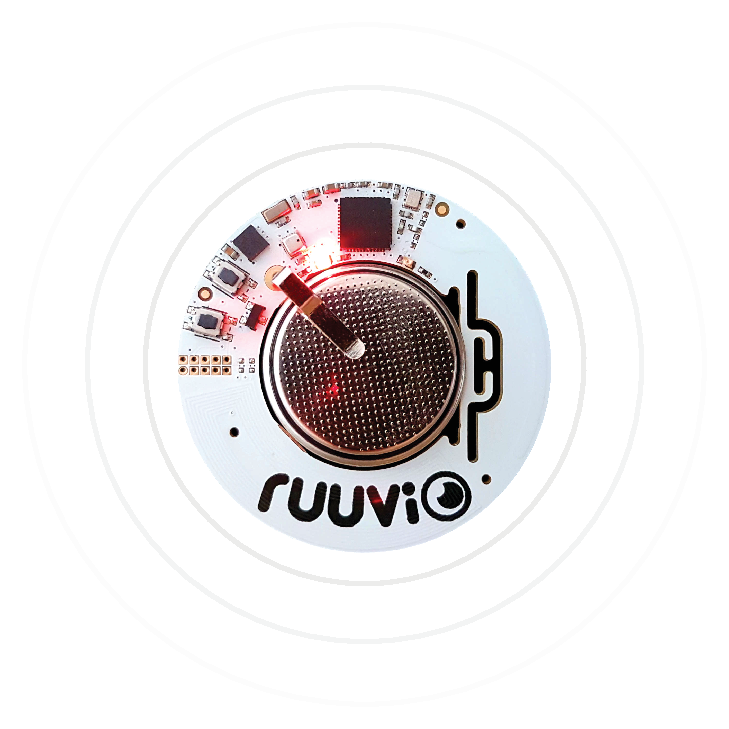
\includegraphics[height=100mm]{ruuvi-tag-rounds.pdf}
};


% Bottom boxes

\node[block, anchor=south, yshift=6mm] (G) at (L.south) {
  \centering \mlfont{11}{\href{http://ruuvitag.com}{ruuvitag.com}}
};

\node[block, anchor=south, yshift=19mm] (F) at (L.south) {
  \includegraphics[height=7mm]{ruuvi-logo-white} % revert white logo
};

\node[block, anchor=south, yshift=22mm, text depth=3pt] (E) at (F.south) {
  \centering \orfont{14}{COMING SOON TO KICKSTARTER!}
};

\draw[line width=2pt, yellow] ($(E.south west)+(4pt,0)$) |- ($(E.south east)-(4pt,0)$);

\end{scope}



% Rigth column
% ------------

% Background image of the column
\node[col=\rightcolwidth, fill=black] (R) at ($(current page.south west)+(\leftcolwidth,0)$) {
  % \includegraphics[height=\paperheight]{col_right}
};

\begin{scope}[x={(R.south west)}, y={(R.north east)}]

% Top boxes

$body$

\node[block, text width=0.915\rightcolwidth, anchor=north west, xshift=7mm, yshift=-8mm] (A) at (R.north west) {
  \olfont{14}{SOON AVAILABLE FOR EVERYONE:}\\[10pt]
  \orfont{20}{Open-Source Bluetooth 4.2 Sensor Beacon Goes to Kickstarter!} \\[18pt]
  
  \orfont{14}{WHAT IS IT?}\\[12pt]
  
  \mlfont{11}{\baselineskip=14pt The Internet of Things, beacons and Physical Web are today’s hot topics. We will be surrounded by small intelligent sensor nodes that analyze the environment and offer people more content on their smartphones. Lots of traditional proximity beacon products are already available out there, but what the market is truly lacking is an open sourced device.\\[10pt]
We decided to change this. A year ago we started a design process with one goal: to create a superior open-source sensor beacon platform to fulfill the needs of both developers and makers. We managed to create one of the most advanced Bluetooth sensor products in the world. Now what we want, more than anything, is to make it available for everyone. To make this a reality we are launching a global Kickstarter campaign for this project.\\[14pt]}
  
  \orfont{14}{HOW TO USE IT?}\\[12pt]
  
  \mlfont{11}{\baselineskip=14pt RuuviTag can act as a standard Eddystone/iBeacon proximity beacon but it has the potential to be so much more. By having a way to measure temperature, humidity, air pressure and acceleration it’s possible to cover several use cases. No need to worry about charging the device because the battery life lasts up to 10 years.\\[10pt]
The device can be easily adjusted to cover different kinds of needs. Use it as a remote weather station with readings that can be pulled up on your mobile phone, attach one to your bicycle so you can be notified if someone moves it or tell it to broadcast a Physical Web address. There are endless possibilities for its set up. No programming tools or advanced technical knowledge is required. But, because everything is open-source, the opportunities are limitless.\\[14pt]}
  
  \orfont{14}{SUPPORTING EDUCATION}\\[12pt]
  
  \mlfont{11}{\baselineskip=14pt The Tag is also a perfect tool for education. We want to give RuuviTags free for educational purposes to schools and universities around the world. The more the campaign grows, more free devices we can ship out.\\[10pt]
For more info and to stay informed, check our website and join mailing list: ruuvitag.com\\
You can also reach us via email: info@ruuvi.com}
};
\end{scope}

\end{tikzpicture}

$for(include-after)$
$include-after$
$endfor$

\end{document}
